\par\Needspace{10\baselineskip}
\section{路径积分}
\label{sec:multivariable-path-integration}

区域积分累计的是铺满一块区域的量，许多问题却只沿一条曲线累计。一根弯曲细铁丝的质量由各处的线密度和铁丝长度决定；把物体沿一条路线推过去，推力做的功不仅取决于力的大小和路线长度，还取决于力与前进方向的夹角。
两类问题都沿曲线累计，被积对象却不同：线密度在每一点只给出一个数，是标量函数；力在每一点给出一个带方向的量，是向量场。

相应地有两种路径积分。第一类路径积分把曲线切成小段，用每段上的函数值乘这段的实际长度再相加，铁丝质量就是这样算出的；它不关心沿哪个方向走过曲线。
第二类路径积分在每一小段上先取力与这段有向位移的内积，只保留力沿前进方向的分量，再把这些数相加；反向行走时每段位移都反号，积分也随之变号。

两种积分都要先用参数描述曲线，因此本节先说明路径与弧长，再分别讨论两类积分的定义、性质和计算。
最后研究力沿路径做的功什么时候只取决于起点和终点、而与中间的路线无关，这对应物理中保守力与势能的关系。
本节的参数积分都是一元勒贝格积分\scite{math-openstax-calculus3}。

\subsection{参数路径与弧长}
\label{sec:multivariable-line-integrals}

描述一次行进，需要知道每个时刻所在的位置。位置随时间连续变化，就得到一条路径；位置对时间的导数是速度，速度的大小称为速率。速率恒定时，速率乘经过的时间就是走过的路程。
本小节先给出路径的定义，再用折线逼近说明：速率随时间变化时，路程等于速率对时间的积分。

\subsubsection{路径的定义}

\paragraph{参数化路径}

不妨把参数$t$看成时间，把$\gamma(t)$看成一个质点在时刻$t$所在的位置。同一组位置可以走得快或慢，可以从任一端出发，也可以来回走好几遍；只记下经过了哪些点，就会丢失这些信息。用区间到空间的连续映射描述行进过程，位置和先后次序就一起保留了下来。
\begin{definition}[路径]
设$a<b$。连续映射$\gamma:[a,b]\to\mathbb R^d$称为一条\term{路径}（path），$\gamma(a)$和$\gamma(b)$分别为起点和终点；若两者相等，称为闭路径。
集合$C=\gamma([a,b])$称为路径的像。
\end{definition}

像集$C$只记录质点经过的位置，参数$t$还规定了经过的先后次序，所以同一个像集可以对应行进方式完全不同的路径。
\begin{example}[同一条对角线段上的三条路径]
\label{ex:analysis-diagonal-segment-paths}
以下三条平面路径的像都是连接$(0,0)$与$(1,1)$的对角线段：
\begin{itemize}
 \item $\gamma(t)=(t,t)^\top$，$0\leq t\leq1$，从$(0,0)$走到$(1,1)$，速度为$(1,1)^\top$；
 \item $\eta(u)=(u/2,u/2)^\top$，$0\leq u\leq2$，同样从$(0,0)$走到$(1,1)$，速度减半为$(1/2,1/2)^\top$，用时加倍；
 \item $\rho(t)=(t,t)^\top$（$0\leq t\leq1$）、$\rho(t)=(2-t,2-t)^\top$（$1\leq t\leq2$），先走到$(1,1)$再原路返回。
\end{itemize}
$\gamma$与$\eta$只是快慢不同，线段上每个点都恰好经过一次。$\rho$的像仍是这条线段，但每个内点被经过两次：去程一次，回程一次。
\end{example}

后面会看到，两种路径积分对$\gamma$与$\eta$都给出相同结果；沿$\rho$按长度累计时，结果是沿$\gamma$的两倍，按有向位移累计时，去程与回程恰好抵消。
可见路径积分是沿“一次行进”定义的，只知道像集还不能确定它。要计算一根铁丝的质量，应选一条把铁丝恰好走一遍的路径。

\paragraph{分段光滑路径}

示例~\ref{ex:analysis-diagonal-segment-paths}中的往返路径$\rho$在$t=1$处突然掉头，正方形边界在四个角处突然转向。这些位置没有唯一的切线方向，但在每一段直线上速度都存在且连续。为了把折线、多边形边界这类常见路径纳入计算，允许路径在有限个参数点处分段。
\begin{definition}[分段光滑路径]
若存在分割$a=t_0<t_1<\cdots<t_n=b$，使$\gamma$在每个$[t_{j-1},t_j]$上为$C^1$映射，称$\gamma$为分段$C^1$路径，也称分段光滑路径。
若每段内部还满足$\gamma'(t)\neq\bm0$，称该路径分段正则。
\end{definition}

这里“在闭区间$[t_{j-1},t_j]$上为$C^1$”是指该段内部的导数连续，并能连续延拓到该段的两个端点；相邻两段在公共端点处的导数不必相同。
例如$\rho$在$[0,1]$上的速度为$(1,1)^\top$，在$[1,2]$上的速度为$(-1,-1)^\top$。两段在$t=1$处的速度不同，但各自连续，所以$\rho$是分段$C^1$路径。

本节的路径积分都在分段$C^1$路径上定义。折点只有有限个，而参数区间中的有限点集测度为零，所以折点处的速度取什么值不影响参数积分。
分段正则要求每段内部速度不为零，排除了质点在某段中途停住的情形。本节的积分并不要求路径正则；后面用到单位切向量时，只在速度非零处使用它。

\subsubsection{路径的长度}

\paragraph{弧长}

测量一条弯曲道路的长度时，可以在路上依次插几根标杆，量出相邻标杆之间的直线距离再相加。每段直线距离都不超过对应那段路的实际长度，所以这样得到的折线长度不会超过道路长度；在两根标杆之间再插一根，由三角不等式，新折线的长度不会变短。标杆越密，折线越贴近道路，因此把实际长度定义为所有内接折线长度的上确界。
\begin{definition}[路径的弧长]
路径$\gamma:[a,b]\to\mathbb R^d$的弧长定义为
\[
 \ell(\gamma)=\sup_{a=t_0<\cdots<t_n=b}
 \sum_{j=1}^n\lVert\gamma(t_j)-\gamma(t_{j-1})\rVert_2.
\]
上确界取遍$[a,b]$的全部有限分割；若此值有限，称路径可求长。
\end{definition}

这个定义只用到路径上点的位置，不需要导数，所以任何连续路径都可以讨论它是否可求长。对分段光滑路径，弧长还可以用速度直接计算。在一小段参数区间$[t_{j-1},t_j]$上，质点的位移近似为速度乘时间：
$\gamma(t_j)-\gamma(t_{j-1})\approx\gamma'(t_{j-1})(t_j-t_{j-1})$，
所以这一小段的长度近似为速率$\lVert\gamma'(t_{j-1})\rVert_2$乘时间，汽车里程表正是这样累计路程的。把这些乘积相加并令分割变细，就得到下面的公式。
\begin{theorem}[分段光滑路径的弧长]
若$\gamma:[a,b]\to\mathbb R^d$分段$C^1$，则它可求长，且
\[
 \ell(\gamma)=\int_a^b\lVert\gamma'(t)\rVert_2\,\mathrm dt.
\]
\end{theorem}
\begin{proof}
加入分点不会使折线变短，所以计算上确界时只需考虑包含全部折点的分割；这样的折线长度按光滑段相加，弧长也按段相加。因此只需在一段$C^1$区间上证明，再把各段的等式相加。证明分两步：先说明任何折线都不比速度积分长，再说明足够细的折线与速度积分相差任意小。

第一步。对该段中的$\alpha<\beta$，由各坐标分量的一元基本定理，
$\gamma(\beta)-\gamma(\alpha)=\int_\alpha^\beta\gamma'(t)\,\mathrm dt$，这里向量的积分表示对各分量分别积分。
若弦$\gamma(\beta)-\gamma(\alpha)$非零，取它方向上的单位向量$\bm u$，则由Cauchy--Schwarz不等式
\[
 \lVert\gamma(\beta)-\gamma(\alpha)\rVert_2
 =\bm u^\top\bigl(\gamma(\beta)-\gamma(\alpha)\bigr)
 =\int_\alpha^\beta\bm u^\top\gamma'(t)\,\mathrm dt
 \leq\int_\alpha^\beta\lVert\gamma'(t)\rVert_2\,\mathrm dt;
\]
弦为零时这个不等式直接成立。同样的推理说明，任何连续向量值函数$\bm v$都满足$\lVert\int_\alpha^\beta\bm v\,\mathrm dt\rVert_2\leq\int_\alpha^\beta\lVert\bm v\rVert_2\,\mathrm dt$。
对任意分割把各段弦长相加，可知任意内接折线的长度都不超过$\int_a^b\lVert\gamma'\rVert_2\,\mathrm dt$，所以上确界也不超过它。

第二步。$\gamma'$在紧区间上一致连续。给定$\varepsilon>0$，取足够细的分割，使每个小区间上任意两点的$\gamma'$相距小于$\varepsilon$，并记$\Delta t_j=t_j-t_{j-1}$。
在第$j$个小区间上，
\[
 \gamma(t_j)-\gamma(t_{j-1})-\gamma'(t_{j-1})\Delta t_j
 =\int_{t_{j-1}}^{t_j}\bigl(\gamma'(t)-\gamma'(t_{j-1})\bigr)\,\mathrm dt,
\]
由第一步的范数不等式，它的范数不超过$\varepsilon\Delta t_j$；于是这一段的弦长与$\lVert\gamma'(t_{j-1})\rVert_2\Delta t_j$之差不超过$\varepsilon\Delta t_j$。
同一小区间上，$\int\lVert\gamma'\rVert_2\,\mathrm dt$与$\lVert\gamma'(t_{j-1})\rVert_2\Delta t_j$的差也不超过$\varepsilon\Delta t_j$。
两项相加后对$j$求和，速度积分与这条折线长度的差不超过$2\varepsilon(b-a)$，所以上确界不小于速度积分减$2\varepsilon(b-a)$。令$\varepsilon\downarrow0$，得到反向不等式。
\end{proof}

用这个公式可以计算示例~\ref{ex:analysis-diagonal-segment-paths}中三条路径的长度，并检验圆周长公式。
\begin{example}[对角线段与圆周的弧长]
对角线段$\gamma(t)=(t,t)^\top$，$0\leq t\leq1$，速度为$(1,1)^\top$，速率为$\sqrt2$，所以$\ell(\gamma)=\int_0^1\sqrt2\,\mathrm dt=\sqrt2$。两个坐标各变化$1$，走过的距离却不是$1+1=2$，而是斜边的长度。

慢速路径$\eta$的速率为$\sqrt2/2$，用时为$2$，长度为$\int_0^2(\sqrt2/2)\,\mathrm du=\sqrt2$。往返路径$\rho$在两段上的速率都是$\sqrt2$，总用时为$2$，长度为$2\sqrt2$。

半径为$r$的圆周可以参数化为$t\mapsto(r\cos t,r\sin t)^\top$，$0\leq t\leq2\pi$。速度为$(-r\sin t,r\cos t)^\top$，速率恒为$r$，长度为$\int_0^{2\pi}r\,\mathrm dt=2\pi r$，与圆周长公式一致。
\end{example}

$\gamma$与$\eta$的长度相同，因为速率减半恰好被用时加倍抵消；$\rho$的长度是$\gamma$的两倍，因为弧长把经过的次数也计算在内。

记$s(t)=\int_a^t\lVert\gamma'(u)\rVert_2\,\mathrm du$为截至时刻$t$累计走过的路程，它就是里程表在时刻$t$的读数。在每个光滑段内部，$s$对$t$的导数是速率$\lVert\gamma'(t)\rVert_2$，因此常把长度权重简写为
$\mathrm ds=\lVert\gamma'(t)\rVert_2\,\mathrm dt$，读作“一小段时间$\mathrm dt$内走过的一小段路程”。

\subsection{第一类路径积分}

第一类路径积分的被积对象是定义在曲线上的标量函数，例如铁丝各处的线密度或一条道路沿线各处的温度。每一小段的贡献是函数值乘这一小段的实际长度，因此它只需要路程这一个权重，不涉及方向。

\subsubsection{定义与可积性}

\paragraph{按弧长的积分}

设一根铁丝沿路径$\gamma$放置，$h(\bm x)$是它在点$\bm x$处的线密度，即单位长度的质量。线密度为常数时，质量等于密度乘长度；密度随位置变化时，把铁丝切成许多小段，每段上的密度近似为常数。
在参数小区间$[t_{j-1},t_j]$对应的一段上取一个时刻$\xi_j$，这段的质量约为
\[
 h(\gamma(\xi_j))\,\lVert\gamma'(\xi_j)\rVert_2\,(t_j-t_{j-1}),
\]
即“该处密度”乘“该段长度”。把各段相加，就得到参数区间上函数$h(\gamma(t))\lVert\gamma'(t)\rVert_2$的积分和，所以用这个函数的一元积分定义沿路径的累计。采用勒贝格积分，还能处理沿路径可测而不连续的标量函数。
\begin{definition}[第一类路径积分]
设$\gamma:[a,b]\to\mathbb R^d$分段$C^1$，$h:C\to\mathbb R$，其中$C=\gamma([a,b])$，且$h\circ\gamma$在参数区间上勒贝格可测。
若$h\geq0$，定义\term{第一类路径积分}（scalar line integral）为
\begin{equation}
 \int_\gamma h\,\mathrm ds
 =\int_a^b h(\gamma(t))\lVert\gamma'(t)\rVert_2\,\mathrm dt,
 \label{eq:analysis-scalar-line-integral}
\end{equation}
允许取$+\infty$。对一般有符号$h$，本节称它沿$\gamma$可积，是指
\[
 \int_a^b |h(\gamma(t))|\lVert\gamma'(t)\rVert_2\,\mathrm dt<\infty;
\]
此时由正负部分之差定义积分，式~\eqref{eq:analysis-scalar-line-integral}仍成立并取有限值。
\end{definition}

这个积分有几种常见读法。取$h=1$，积分就是弧长$\ell(\gamma)$；$h$是非负线密度时，积分是铁丝的总质量。

若$\ell(\gamma)>0$，比值
\[
 \bar h=\frac1{\ell(\gamma)}\int_\gamma h\,\mathrm ds
\]
是$h$沿曲线按长度的平均值：沿一条道路每隔相同路程记录一次温度再求平均，记录越密，结果越接近$\bar h$。
这里的平均按路程加权，而不按参数时间加权。若一辆车在某段路上开得很慢，按时间平均会让这段路的温度占更大比重，按路程平均则不受车速影响。

用一根密度不均匀的半圆铁丝可以说明质量和平均线密度的计算。
\begin{example}[上半圆铁丝的质量与平均线密度]
\label{ex:analysis-semicircle-wire}
沿上半单位圆$\gamma(t)=(\cos t,\sin t)^\top$，$0\leq t\leq\pi$，放一根铁丝，线密度为$h(x,y)=y$，即越高的地方越重。速度为$(-\sin t,\cos t)^\top$，速率恒为$1$，所以总质量为
\[
 \int_\gamma y\,\mathrm ds=\int_0^\pi\sin t\,\mathrm dt=2.
\]
铁丝长度为$\pi$，平均线密度为$\bar h=2/\pi\approx0.64$。两端$(\pm1,0)$处密度为零，顶点$(0,1)$处密度为$1$，平均值落在两者之间。
\end{example}
这条参数化的速率恒为$1$，参数时间与路程同步增长，所以按时间平均也得到$2/\pi$；速率不恒定时，两种平均一般不同。

若$h$在像集$C$上连续，由于$C$是紧区间在连续映射下的像，也是紧集，$h$在$C$上有界，绝对积分不超过$\sup_C|h|\,\ell(\gamma)<\infty$，因而$h$沿$\gamma$可积。连续性是方便的充分条件，并非定义本身的要求。

定义要求的是$h$在曲线上的实际取值，以及它与参数复合后的可测性。仅知道$h$作为平面函数勒贝格可积，并不能确定这个积分：平面上几乎处处相等的两个函数，沿同一条曲线的积分可以不同。
\begin{example}[平面积分为零而沿线段的积分为一]
令$h(x,y)=\mathbb I\{y=0\}$，它只在$x$轴上取$1$，在其余位置取$0$。$x$轴的平面测度为零，所以$h$与零函数在平面上几乎处处相等，$h$在平面上的积分为$0$。
沿$\gamma(t)=(t,0)^\top$，$0\leq t\leq1$，有$h(\gamma(t))=1$且速率为$1$，所以$\int_\gamma h\,\mathrm ds=1$；零函数沿同一路径的积分却是$0$。
\end{example}
原因是曲线本身的面积为零：改变平面函数在一个零面积集合上的值，不影响区域积分，却可能完全改变沿这个集合的路径积分。

\subsubsection{积分的基本性质}

下面各条性质中的有符号函数都假设沿所讨论的路径可积。把定义式~\eqref{eq:analysis-scalar-line-integral}代入一元勒贝格积分的相应性质，就逐项得到这些结论；用铁丝质量来读，每条性质都有直接的含义。

\paragraph{加法}

若$h,k$沿$\gamma$可积，则$h+k$也沿$\gamma$可积，且
\[
 \int_\gamma(h+k)\,\mathrm ds=\int_\gamma h\,\mathrm ds+\int_\gamma k\,\mathrm ds.
\]
绝对可积性由$|h+k|\leq|h|+|k|$保证，等式来自一元积分的加法。若铁丝由两种材料叠合而成，总质量等于两种材料各自的质量之和。

\paragraph{减法}

把$k$换成$-k$，它同样沿$\gamma$可积，由加法得到
\[
 \int_\gamma(h-k)\,\mathrm ds=\int_\gamma h\,\mathrm ds-\int_\gamma k\,\mathrm ds.
\]
两个积分都是有限数，所以相减时不会出现$\infty-\infty$。

\paragraph{数乘}

若$c\in\mathbb R$且$h$沿$\gamma$可积，则
\[
 \int_\gamma ch\,\mathrm ds=c\int_\gamma h\,\mathrm ds.
\]
把每一小段上的密度同时放大$c$倍，总质量也放大$c$倍。

\paragraph{路径拼接}

若$\gamma_1$的终点是$\gamma_2$的起点，记先走$\gamma_1$、再走$\gamma_2$的拼接路径为$\gamma_1*\gamma_2$。$h$沿两条路径分别可积时，
\[
 \int_{\gamma_1*\gamma_2}h\,\mathrm ds
 =\int_{\gamma_1}h\,\mathrm ds+\int_{\gamma_2}h\,\mathrm ds.
\]
拼接路径的参数区间由两段参数区间首尾相接而成，等式来自一元积分对区间的可加性。逐段计算折线和多边形边界上的积分，依据的正是这个等式。

两段路径有重叠部分时，重叠部分的贡献会计入两次。示例~\ref{ex:analysis-diagonal-segment-paths}中的往返路径$\rho$由去程$\gamma$与原路返回的一段拼成；返回段$(2-t,2-t)^\top$，$1\leq t\leq2$，经换元$u=2-t$化为$\gamma$上的同一个积分，所以沿$\rho$的积分是沿$\gamma$的两倍。

\paragraph{重参数化与方向无关}

同一根铁丝无论从哪一端开始称量、量得快还是慢，质量都不变。数学上，改变快慢和方向都可以用换参数表示：设$t=\sigma(u)$是两个参数区间之间单调、端点相配的分段$C^1$微分同胚，新路径$\gamma\circ\sigma$在“时刻”$u$位于$\gamma(\sigma(u))$。
链式法则给出新速度$(\gamma\circ\sigma)'(u)=\gamma'(\sigma(u))\sigma'(u)$，所以新速率为
$\lVert\gamma'(\sigma(u))\rVert_2|\sigma'(u)|$。代入定义并用一元换元公式$t=\sigma(u)$，得到
\[
 \int_{\gamma\circ\sigma}h\,\mathrm ds=\int_\gamma h\,\mathrm ds.
\]

走得慢时速率变小，但用时按同一比例变长，乘积不变。$\sigma$递减时路径反向，绝对值$|\sigma'|$仍给出非负的长度权重，所以反向行进也不改变第一类积分。
在示例~\ref{ex:analysis-diagonal-segment-paths}中，$\eta=\gamma\circ\sigma$，其中$\sigma(u)=u/2$，$0\leq u\leq2$，所以沿$\eta$与沿$\gamma$的第一类积分相同，弧长都是$\sqrt2$。换参数只改变快慢和方向，不改变经过的次数，所以往返路径$\rho$不是$\gamma$的重参数化。

\paragraph{单调性}

若在路径上处处有$h\leq k$，则
\[
 \int_\gamma h\,\mathrm ds\leq\int_\gamma k\,\mathrm ds.
\]
这是因为长度权重$\lVert\gamma'\rVert_2$非负，被积函数的大小关系乘以权重后保持不变。密度处处较小的铁丝，总质量也较小。

\paragraph{绝对值不等式}

由一元积分的绝对值不等式可得
\[
 \left|\int_\gamma h\,\mathrm ds\right|
 \leq\int_\gamma|h|\,\mathrm ds
 \leq\sup_C|h|\,\ell(\gamma).
\]
$h$有界时，最后一个不等式给出有限的上界：累计量的绝对值不超过函数绝对值的上确界乘路径长度。例如在示例~\ref{ex:analysis-semicircle-wire}中，密度$y$不超过$1$，质量$2$确实不超过$1\cdot\pi$。

\subsubsection{积分的计算}

计算第一类路径积分分三步：给曲线选一条把它恰好走一遍的参数化；把$h(\gamma(t))$乘速率$\lVert\gamma'(t)\rVert_2$；在参数区间上做一元积分，有折点时在折点两侧分别计算再相加。
先在示例~\ref{ex:analysis-diagonal-segment-paths}的对角线段上积分一个线性函数。
\begin{example}[沿对角线段积分$x+y$]
取$\gamma(t)=(t,t)^\top$，$0\leq t\leq1$，$h(x,y)=x+y$。沿路径有$h(\gamma(t))=2t$，速率为$\sqrt2$，所以
\[
 \int_\gamma h\,\mathrm ds=\int_0^1 2t\cdot\sqrt2\,\mathrm dt=\sqrt2.
\]
线段长为$\sqrt2$，平均值为$\sqrt2/\sqrt2=1$，恰是$h$在线段中点$(1/2,1/2)$的值，因为$h$沿这条线段随路程线性变化。
\end{example}
若漏掉速率而只计算$\int_0^12t\,\mathrm dt=1$，得到的是按参数时间的累计，比按长度的累计少了速率因子$\sqrt2$。第一类路径积分也不是线段下方某块平面区域的面积：区域积分按面积加权，这里的权重是沿线段的长度。

许多平面曲线写成函数图像$y=\psi(x)$。设$\psi$在$[a,b]$上为$C^1$，沿$x$递增的图像路径$\gamma(x)=(x,\psi(x))^\top$，$a\leq x\leq b$，以$x$本身作参数，速度为$(1,\psi'(x))^\top$，于是
\[
 \int_\gamma h\,\mathrm ds
 =\int_a^b h(x,\psi(x))\sqrt{1+\psi'(x)^2}\,\mathrm dx.
\]
根号是图像路径的速率：自变量前进$\mathrm dx$时，曲线同时升高约$\psi'(x)\,\mathrm dx$，斜边长约为$\sqrt{1+\psi'(x)^2}\,\mathrm dx$。曲线越陡，同一个$\mathrm dx$对应的路程越长，因此不能只写$\mathrm dx$。

用这个公式可以计算一段抛物线铁丝的质量。
\begin{example}[抛物线铁丝的质量]
沿抛物线段$y=x^2$，$0\leq x\leq1$，放一根铁丝，线密度为$h(x,y)=x$。这里$\psi(x)=x^2$，$\psi'(x)=2x$，速率为$\sqrt{1+4x^2}$。令$w=1+4x^2$，则$\mathrm dw=8x\,\mathrm dx$，$w$从$1$变到$5$，所以
\[
 \int_\gamma x\,\mathrm ds=\int_0^1x\sqrt{1+4x^2}\,\mathrm dx
 =\frac18\int_1^5\sqrt w\,\mathrm dw=\frac{5\sqrt5-1}{12}\approx0.85.
\]
\end{example}
若漏写根号，只会得到$\int_0^1x\,\mathrm dx=1/2$，丢掉了曲线变陡后多出的长度。

\subsection{第二类路径积分}

第一类积分只问“每段有多长”，做功问题还要问“这段朝哪个方向走”。推一辆车时，力与前进方向一致才完全用于推动，力与前进方向垂直时不做功，力与前进方向相反时做负功。描述这种累计，需要先说明“每一点有一个力”是什么意思。

\subsubsection{定义与可积性}

\paragraph{向量场}

力在空间中随位置变化：地面附近的重力处处竖直向下，太阳对行星的引力指向太阳且随距离减弱。河流中的水在每一点有一个流速，流速同样带有大小和方向。这类对象在每个位置给出一个与位置同维的向量。
\begin{definition}[向量场]
设$U\subseteq\mathbb R^d$。映射$\bm F:U\to\mathbb R^d$称为$U$上的\term{向量场}（vector field）。
\end{definition}

向量场的输入是位置，输出是放在该位置的一个向量，常画成从该点出发的箭头。下面是三个平面例子：
\begin{itemize}
 \item 常向量场$\bm F(x,y)=(0,-mg)^\top$描述地面附近质量为$m$的物体所受重力，其中$g$是重力加速度，箭头处处竖直向下、长度相同；
 \item $\bm F(x,y)=(x,y)^\top$的箭头从原点向外，离原点越远越长；
 \item $\bm F(x,y)=(-y,x)^\top$的箭头与以原点为圆心的圆相切，按逆时针方向，长度等于到原点的距离。它是绕原点以角速度$1$旋转的圆盘上各点的速度，本节称它为旋转场。
\end{itemize}
旋转场与位置向量处处垂直，因为$(-y)\cdot x+x\cdot y=0$。

\paragraph{有向线积分}

先看最简单的情形：常力$\bm F$把物体沿直线移动了位移$\Delta\bm r$。中学物理中的功是$\lVert\bm F\rVert_2\lVert\Delta\bm r\rVert_2\cos\theta$，其中$\theta$是力与位移的夹角，它正是内积$\bm F^\top\Delta\bm r$。把力分解为沿位移方向和垂直于位移方向的两部分，只有前一部分做功：$\theta<\pi/2$时功为正，$\theta=\pi/2$时为零，$\theta>\pi/2$时为负。

路线弯曲、力随位置变化时，把路径切成许多小段。参数小区间$[t_{j-1},t_j]$上的位移近似为$\gamma'(\xi_j)(t_j-t_{j-1})$，力近似为常力$\bm F(\gamma(\xi_j))$，这段的功约为
\[
 \bm F(\gamma(\xi_j))^\top\gamma'(\xi_j)\,(t_j-t_{j-1}).
\]
各段相加就是参数区间上函数$\bm F(\gamma(t))^\top\gamma'(t)$的积分和。这里乘的是速度向量本身，不是速率，所以位移的方向保留在被积函数中。
\begin{definition}[第二类路径积分]
设$\gamma:[a,b]\to U$分段$C^1$，$\bm F:U\to\mathbb R^d$为向量场。
若$\bm F\circ\gamma$的每个分量勒贝格可测，且$t\mapsto\bm F(\gamma(t))^\top\gamma'(t)$绝对可积，定义\term{第二类路径积分}（vector line integral）为
\begin{equation}
 \int_\gamma\bm F\mathbin{\cdot}\mathrm d\bm r
 =\int_a^b\bm F(\gamma(t))^\top\gamma'(t)\,\mathrm dt.
 \label{eq:analysis-vector-line-integral}
\end{equation}
\end{definition}

记号$\mathrm d\bm r$表示一小段有向位移$\gamma'(t)\,\mathrm dt$，$\bm F\cdot\mathrm d\bm r$是这一小段上的功。
在平面中，若$\bm F=(P,Q)^\top$，路径为$\gamma(t)=(x(t),y(t))^\top$，则被积函数是$P\,x'(t)+Q\,y'(t)$，因此积分也写成$\int_\gamma P\,\mathrm dx+Q\,\mathrm dy$：$P\,\mathrm dx$是力的水平分量在水平位移上做的功，$Q\,\mathrm dy$是竖直分量在竖直位移上做的功。三维中再加上第三个分量$R$对应的$R\,\mathrm dz$。

若$\bm F$在路径像集上连续，复合函数$\bm F\circ\gamma$在各光滑段上连续，被积函数在紧参数区间上有界，所以参数积分绝对可积。
更一般地，只要$\bm F\circ\gamma$可测且$\int_a^b\lVert\bm F(\gamma(t))\rVert_2\lVert\gamma'(t)\rVert_2\,\mathrm dt<\infty$，积分就存在，因为内积的绝对值不超过两个范数之积。

两类路径积分可以用单位切向量联系起来。在速度非零处，单位切向量$\bm\tau=\gamma'/\lVert\gamma'\rVert_2$指向前进方向，于是
\[
 \bm F^\top\gamma'\,\mathrm dt=(\bm F^\top\bm\tau)\,\lVert\gamma'\rVert_2\,\mathrm dt=(\bm F^\top\bm\tau)\,\mathrm ds.
\]
$\bm F^\top\bm\tau$是力在前进方向上的分量，称为切向分量。速度为零处，左侧的被积函数为零，右侧的长度权重$\lVert\gamma'\rVert_2$也为零，不必定义$\bm\tau$。所以第二类积分等于切向分量的第一类积分：功等于“沿前进方向的力”乘“走过的路程”再累计。
区别在于，切向分量依赖于行进方向：反向行走时$\bm\tau$变为$-\bm\tau$，切向分量变号，积分也变号；而第一类积分的被积函数与方向无关。

若$\bm F$是流体的速度场，沿闭路径的积分累计的是流速沿这条闭路径的切向分量，称为\term{环流}（circulation）。环流为正，表示流体总体上倾向于沿所选方向绕这条闭路径流动。
例如沿单位圆逆时针行进时，旋转场$(-y,x)^\top$的切向分量处处为$1$，一周的环流是$1\times2\pi=2\pi$。

图~\ref{fig:analysis-process-line-density-work}用同一条线段对照两类积分：左图按长度累计常数密度，右图只累计位移的水平分量。
\begin{figure}[!htbp]
 \centering
 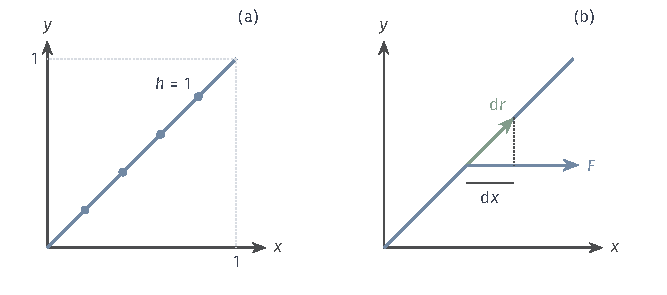
\includegraphics[width=112mm]{figures/01-mathematical-preliminaries-upper/01-mathematical-language-combinatorics-analysis-optimization/tikz/chapter3-concept-processes/line-density-work.pdf}
 \caption{路径均为$\gamma(t)=(t,t)^\top$，$0\leq t\leq1$。(a) 常数线密度$h=1$按弧长累计，得到$\sqrt2$。(b) 常向量场$\bm F=(1,0)^\top$只取位移的水平分量，做功为$1$；图中$\mathrm dx$是$\mathrm d\bm r$的水平投影。相同路径、不同被积对象和权重给出不同积分。}
 \label{fig:analysis-process-line-density-work}
\end{figure}

\subsubsection{积分的基本性质}

下列公式均由内积的线性和一元勒贝格积分的相应性质得到。以下说$\bm F$沿$\gamma$可积，是指定义中的可测性与绝对可积条件成立，因而相应的有向积分有限。前三条说明功对力是线性的，接下来三条说明功怎样随路径的拼接、方向和参数化变化，最后一条估计功的大小。

\paragraph{加法}

若$\bm F$和$\bm G$沿$\gamma$可积，则$\bm F+\bm G$也沿$\gamma$可积，且
\[
 \int_\gamma(\bm F+\bm G)\cdot\mathrm d\bm r
 =\int_\gamma\bm F\cdot\mathrm d\bm r+\int_\gamma\bm G\cdot\mathrm d\bm r.
\]
这里先把两个向量场相加，再与位移取内积。两个力同时作用时，合力做的功等于两个力各自做功之和。

\paragraph{减法}

把$\bm G$换成相反场$-\bm G$，由加法得到
\[
 \int_\gamma(\bm F-\bm G)\cdot\mathrm d\bm r
 =\int_\gamma\bm F\cdot\mathrm d\bm r-\int_\gamma\bm G\cdot\mathrm d\bm r.
\]
可积性保证两个积分都有限，所以可以相减。

\paragraph{数乘}

对实数$c$，有
\[
 \int_\gamma c\bm F\cdot\mathrm d\bm r
 =c\int_\gamma\bm F\cdot\mathrm d\bm r.
\]
力放大$c$倍，功也放大$c$倍；$c<0$时力反向，功变号。路径本身没有改变。

\paragraph{路径拼接}

若$\gamma_1$和$\gamma_2$首尾相接，则
\[
 \int_{\gamma_1*\gamma_2}\bm F\cdot\mathrm d\bm r
 =\int_{\gamma_1}\bm F\cdot\mathrm d\bm r
 +\int_{\gamma_2}\bm F\cdot\mathrm d\bm r.
\]
先走一段再走一段，总功是两段的功之和。因此分段光滑路径可以逐段计算，但每段都必须按这次行进的实际方向参数化。

\paragraph{方向反转}

记反向路径为$\gamma^{-}(u)=\gamma(a+b-u)$，$a\leq u\leq b$，它从$\gamma(b)$出发、沿原路走回$\gamma(a)$。由链式法则，它的速度是$-\gamma'(a+b-u)$，与原速度相反；再用一元换元$t=a+b-u$，得到
\[
 \int_{\gamma^{-}}\bm F\cdot\mathrm d\bm r
 =-\int_\gamma\bm F\cdot\mathrm d\bm r.
\]
顺风骑车时风做正功，沿原路逆风骑回来，风在每一段都做等量的负功。第一类积分反向后不变，因为长度始终非负；有向位移反向则改变符号。
特别地，往返路径$\gamma*\gamma^{-}$上的第二类积分为零，而它的长度是$\gamma$的两倍；示例~\ref{ex:analysis-diagonal-segment-paths}中的$\rho$就是对角线段上的这种往返路径。

\paragraph{重参数化}

若$t=\sigma(u)$为端点相配、严格递增的分段$C^1$微分同胚，则
$(\gamma\circ\sigma)'(u)=\gamma'(\sigma(u))\sigma'(u)$。在参数公式中应用换元$t=\sigma(u)$，得到
\[
 \int_{\gamma\circ\sigma}\bm F\cdot\mathrm d\bm r
 =\int_\gamma\bm F\cdot\mathrm d\bm r.
\]
也就是说，功只取决于经过哪些位置、朝哪个方向经过，与走得快慢无关。
与第一类积分不同，这里乘的是$\sigma'$本身而不是$|\sigma'|$。严格递减的重参数化把路径变成反向路径，换元后积分上下限交换，积分因此变号。重参数化也不改变经过的次数，同一段路重复走两次时，两次的功都会计入。

\paragraph{绝对值不等式}

由积分的三角不等式和Cauchy--Schwarz不等式$|\bm F^\top\bm\tau|\leq\lVert\bm F\rVert_2$可得
\[
 \left|\int_\gamma\bm F\cdot\mathrm d\bm r\right|
 \leq\int_\gamma\lVert\bm F\rVert_2\,\mathrm ds.
\]
功的绝对值不超过力的大小沿路程的累计；当力处处沿前进方向时取等号。若力的大小不超过$M$，路径长为$\ell$，功的绝对值便不超过$M\ell$。
右侧为$+\infty$时，不等式仍成立，但不能用来证明左侧有限。

\subsubsection{积分的计算}

计算第二类路径积分时，按行进方向参数化路径，把场值与速度向量取内积，再做一元积分。与第一类积分相比，这里乘的是速度向量而不是速率。
先用图~\ref{fig:analysis-process-line-density-work}右图中的常力检验这一步骤。
\begin{example}[常力沿对角线段做功]
取常向量场$\bm F=(1,0)^\top$与对角线段$\gamma(t)=(t,t)^\top$，$0\leq t\leq1$。速度为$(1,1)^\top$，被积函数为$1\cdot1+0\cdot1=1$，所以
\[
 \int_\gamma\bm F\cdot\mathrm d\bm r=\int_0^1 1\,\mathrm dt=1.
\]
\end{example}
同一路径的长度为$\sqrt2$。功为$1$而不是$\sqrt2$，是因为水平方向的力只对位移的水平分量做功，而线段的水平跨度是$1$。

再看地面附近的重力。它同样是常向量场，这次让路径任意弯曲。
\begin{example}[重力做功只取决于高度差]
\label{ex:analysis-gravity-work}
设质量为$m$的物体沿分段$C^1$平面路径$\gamma(t)=(x(t),y(t))^\top$，$a\leq t\leq b$，从高度$y(a)$移动到高度$y(b)$，所受重力为$\bm F=(0,-mg)^\top$。被积函数为$\bm F(\gamma(t))^\top\gamma'(t)=-mg\,y'(t)$。在每个光滑段上用一元基本定理，再把各段相加，得到
\[
 \int_\gamma\bm F\cdot\mathrm d\bm r
 =\int_a^b(-mg)\,y'(t)\,\mathrm dt=-mg\bigl(y(b)-y(a)\bigr).
\]
例如质量为$1$千克的物体下降$2$米，即$y(b)-y(a)=-2$，取$g\approx9.8$米每二次方秒，无论沿斜坡还是沿弯曲的滑梯，重力都做功约$9.8\times2=19.6$焦。
\end{example}
被积函数中不含$x'(t)$，水平移动不受重力影响，只有高度变化起作用。这个结果只依赖起点和终点的高度，第~\ref{sec:multivariable-potential-path-independence}节将说明这并非偶然。

对平面图像路径$\gamma(x)=(x,\psi(x))^\top$、$a\leq x\leq b$，其中$\psi$为$C^1$，速度为$(1,\psi'(x))^\top$。$\bm F=(P,Q)^\top$时有
\[
 \int_\gamma\bm F\cdot\mathrm d\bm r
 =\int_a^b\bigl[P(x,\psi(x))+Q(x,\psi(x))\psi'(x)\bigr]\,\mathrm dx.
\]

重力的功与路线无关。下面固定起点和终点，比较两条路线上的功，观察一般向量场是否也如此。
\begin{example}[半圆和直径]
\label{ex:analysis-path-integral-comparison}
取上半圆$\gamma(t)=(\cos t,\sin t)^\top$，$0\leq t\leq\pi$，它从$(1,0)$逆时针走到$(-1,0)$，速度为$(-\sin t,\cos t)^\top$，速率为$1$，故长度$\int_\gamma1\,\mathrm ds=\pi$。另取起点和终点相同的直径$\lambda(t)=(1-2t,0)^\top$，$0\leq t\leq1$，速度为$(-2,0)^\top$。

对常场$(1,0)^\top$，沿上半圆的功为$\int_0^\pi(-\sin t)\,\mathrm dt=-2$，沿直径的功为$\int_0^1(-2)\,\mathrm dt=-2$。两条路线都向左净移动了$2$，水平向右的力在两条路线上做功都是$-2$，恰等于函数$\phi(x,y)=x$在终点与起点的差$-1-1$。

对旋转场$\bm F=(-y,x)^\top$，沿上半圆有$\bm F(\gamma(t))=(-\sin t,\cos t)^\top$，与速度相同，内积为$\sin^2t+\cos^2t=1$，故功为$\pi$：质点一直顺着旋转方向走。
沿直径，$\bm F(\lambda(t))=(0,1-2t)^\top$竖直，而位移水平，内积恒为零，功为$0$。
两条路线端点相同，旋转场做的功却不同。
\end{example}

对常场，功与路线无关；对旋转场，功依赖于路线。沿完整单位圆逆时针一周，质点回到起点，旋转场做功$2\pi$而不是零。图~\ref{fig:analysis-process-rotation-field-paths}画出了旋转场与这两条路线。
\begin{figure}[!htbp]
 \centering
 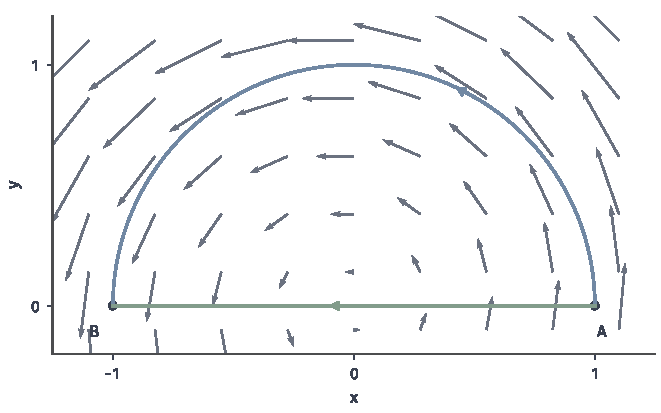
\includegraphics[width=112.0mm]{figures/01-mathematical-preliminaries-upper/01-mathematical-language-combinatorics-analysis-optimization/matplotlib/chapter3-concept-processes/rotation-field-paths.pdf}
 \caption{灰箭头为旋转场$\bm F=(-y,x)^\top$，箭头长度统一缩放为实际场值的$1/4$。两条路径都从$A=(1,0)$到$B=(-1,0)$：蓝色上半圆与场同向，积分为$\pi$；绿色直径上场与位移垂直，积分为零。旋转场处处光滑，端点相同的两条路径上积分仍可不同；下一小节说明势函数给出的路径无关条件。}
 \label{fig:analysis-process-rotation-field-paths}
\end{figure}

\subsection{路径无关与势函数}
\label{sec:multivariable-potential-path-independence}

重力的功只依赖起点和终点的高度，旋转场的功却依赖路线。区别在于：重力的功可以写成某个只依赖位置的量在两端的差，这个量是$-mgy$；旋转场则没有这样的量。
本小节先说明这样的量，即势函数，如何把沿途累计化为端点差；再证明“功与路线无关”反过来也能构造出势函数；最后给出可以直接检查的微分条件，并说明定义域中有洞时，这个条件为什么不再足以保证势函数存在。

\subsubsection{势函数与路径积分}

\paragraph{势函数}

物理中，地面附近质量为$m$的物体在高度$y$处的重力势能为$E_{\mathrm p}(x,y)=mgy$。重力等于势能梯度的相反向量：$-\nabla E_{\mathrm p}=(0,-mg)^\top$。物体下降时势能减少，减少的势能等于重力做的功。
数学中习惯省去负号，取$\phi=-E_{\mathrm p}$，直接要求向量场等于某个标量函数的梯度。
\begin{definition}[势函数]
设$U\subseteq\mathbb R^d$为非空开集，$\bm F:U\to\mathbb R^d$连续。
若存在$\phi\in C^1(U)$使$\bm F=\nabla\phi$，称$\phi$为$\bm F$的\term{势函数}（potential function），称$\bm F$为梯度场，也称保守场。
\end{definition}

梯度指向函数增长最快的方向，所以在梯度非零处，梯度场的箭头指向$\phi$增大的方向，也就是势能$-\phi$减小的方向：重力把物体拉向低处。
例如$\phi(x,y)=x^2+y^2$给出$\bm F(x,y)=(2x,2y)^\top$，箭头从原点向外，因为离原点越远$\phi$越大；常场$(1,0)^\top$的一个势函数是$\phi(x,y)=x$。

给势函数加一个常数，梯度不变，所以势函数不唯一。若$U$还是路径连通的，两个势函数也只能相差一个常数：它们之差的梯度处处为零，路径连通的开集中任意两点都能用域内折线连接，沿折线逐段使用中值公式（定理~\ref{thm:multivariable-scalar-mean-value}），可知这个差在任意两点取值相同。
这与物理中势能的零点可以任选是同一件事：把地面还是桌面取作高度零点，算出的势能差都一样。

“保守”这个名称来自能量守恒。设质量为$m$的质点在力场$\bm F=\nabla\phi$中按牛顿第二定律$m\gamma''(t)=\bm F(\gamma(t))$运动，其中$\gamma$为$C^2$路径。依次用乘积法则、运动方程和链式法则，得到
\[
 \frac{\mathrm d}{\mathrm dt}\Bigl(\tfrac12m\lVert\gamma'(t)\rVert_2^2\Bigr)
 =m\gamma''(t)^\top\gamma'(t)=\nabla\phi(\gamma(t))^\top\gamma'(t)
 =\frac{\mathrm d}{\mathrm dt}\phi(\gamma(t)),
\]
所以动能与势能$-\phi$之和$\frac12m\lVert\gamma'\rVert_2^2-\phi(\gamma)$的导数为零，不随时间变化。最后一个等号已经显示了下面定理的核心：沿路径的功率$\nabla\phi^\top\gamma'$恰是$\phi\circ\gamma$的导数。

\paragraph{路径积分基本定理}

一元基本定理说，导数在区间上的积分等于原函数在两端的差。把势函数与路径复合，得到一元函数$t\mapsto\phi(\gamma(t))$，它的导数恰是第二类路径积分的被积函数，因此一元基本定理直接给出端点差。
直观上，每一小段的功$\nabla\phi^\top\Delta\bm r$近似等于$\phi$在这一小段上的增量，这些增量相加时中间各项逐一抵消，只剩终点值减起点值。
\begin{theorem}[路径积分基本定理]
设$U\subseteq\mathbb R^d$为开集，$\phi\in C^1(U)$，$\gamma:[a,b]\to U$分段$C^1$。则
\begin{equation}
  \int_{\gamma}\nabla\phi\mathbin{\cdot}\mathrm{d}\bm{r}
  =\phi(\gamma(b))-\phi(\gamma(a)).
\label{eq:analysis-line-integral-gradient}
\end{equation}
\end{theorem}
\begin{proof}
在每个光滑参数段$[t_{j-1},t_j]$上，链式法则给出
\[
 (\phi\circ\gamma)'(t)=\nabla\phi(\gamma(t))^\top\gamma'(t).
\]
右侧是连续函数的复合与乘积，在该段上连续，所以对该段使用一元基本定理，得到
$\int_{t_{j-1}}^{t_j}\nabla\phi(\gamma(t))^\top\gamma'(t)\,\mathrm dt=\phi(\gamma(t_j))-\phi(\gamma(t_{j-1}))$。
对$j=1,\dots,n$相加，中间端点的值一正一负逐一抵消，只剩$\phi(\gamma(b))-\phi(\gamma(a))$。
\end{proof}

用势能$E_{\mathrm p}=-\phi$来读，式~\eqref{eq:analysis-line-integral-gradient}说：保守力沿任何路线做的功都等于起点势能减终点势能，即势能的下降量。示例~\ref{ex:analysis-gravity-work}的重力做功就是$\phi(x,y)=-mgy$的情形。

这个定理有两个直接推论。第一，梯度场的积分只依赖端点：两条端点相同的路线，功相同。第二，闭路径的起点与终点重合，所以梯度场沿任意闭路径的积分为零：把书从地上拿到桌上再放回地上，重力在全过程中做的总功为零。
方向反转时端点交换，端点差变号，这与第二类积分的方向反转性质一致。

知道势函数后，计算路径积分不必代入参数。
\begin{example}[用势函数计算沿半圆的积分]
取$\bm F=(2x,2y)^\top$，它的势函数为$\phi(x,y)=x^2+y^2$。路径取示例~\ref{ex:analysis-path-integral-comparison}中的上半圆$\gamma(t)=(\cos t,\sin t)^\top$，$0\leq t\leq\pi$，从$(1,0)$走到$(-1,0)$。由式~\eqref{eq:analysis-line-integral-gradient}，
\[
 \int_\gamma\bm F\cdot\mathrm d\bm r=\phi(-1,0)-\phi(1,0)=1-1=0.
\]
直接代入参数也得到同样结果：$\bm F(\gamma(t))^\top\gamma'(t)=2\cos t\,(-\sin t)+2\sin t\cos t=0$。这个场在圆周上处处沿半径方向，与切线垂直。
\end{example}

第二个推论还可以用来否定势函数的存在。旋转场沿单位圆逆时针一周做功$2\pi\neq0$，所以它在$\mathbb R^2$上没有势函数。

\subsubsection{路径无关的等价判别}

\paragraph{路径无关}

路径积分基本定理说明，有势函数就能推出功与路线无关。要讨论反方向，先把“与路线无关”说准确。比较同一对端点间的不同路线，需要域内任意两点都能用路径连接；对欧氏开集，路径连通时任意两点之间还能选到域内的折线，因而能选到分段光滑路径。
\begin{definition}[路径无关]
设$U\subseteq\mathbb R^d$为非空、开且路径连通的集合，$\bm F:U\to\mathbb R^d$连续。
若对任意$\bm a,\bm b\in U$及域内从$\bm a$到$\bm b$的任意两条分段$C^1$路径，第二类路径积分都相等，称$\bm F$的路径积分与路径无关。
\end{definition}

反方向的想法来自物理中定义势能的办法：选定一个参考点作为势能零点，把力从参考点到某点所做的功取负号，作为该点的势能。只有当这个功与所选路线无关时，这样定义的势能才是一个确定的数。下面的定理说明，路径无关、闭路径积分为零与势函数存在三者等价。
\begin{theorem}[路径无关的等价条件]
设$U\subseteq\mathbb R^d$非空、开且路径连通，$\bm F:U\to\mathbb R^d$连续。下列条件等价：
\begin{enumerate}
 \item 存在$\phi\in C^1(U)$使$\nabla\phi=\bm F$；
 \item $\bm F$的路径积分与路径无关；
 \item 域内每条分段$C^1$闭路径的积分都为零。
\end{enumerate}
\end{theorem}
\begin{proof}
条件1推出条件2，是路径积分基本定理的第一个推论。
条件2推出条件3：设$\gamma$是从$\bm a$出发回到$\bm a$的闭路径。停在$\bm a$不动的常值路径也从$\bm a$到$\bm a$，它的速度为零，积分为零；由路径无关，$\gamma$上的积分也为零。
条件3推出条件2：设$\gamma_1,\gamma_2$都从$\bm a$到$\bm b$。先沿$\gamma_1$走到$\bm b$，再沿$\gamma_2$的反向路径$\gamma_2^-$走回$\bm a$，拼成闭路径$\gamma_1*\gamma_2^-$。由拼接和方向反转性质，
\[
 0=\int_{\gamma_1*\gamma_2^-}\bm F\cdot\mathrm d\bm r
 =\int_{\gamma_1}\bm F\cdot\mathrm d\bm r-\int_{\gamma_2}\bm F\cdot\mathrm d\bm r.
\]

最后由条件2构造势函数。固定参考点$\bm a\in U$，对每个$\bm x\in U$，取域内任意一条从$\bm a$到$\bm x$的分段$C^1$路径，令$\phi(\bm x)$为沿它的积分。路径无关保证这个数不依赖所选路线。
下面计算偏导数。因为$U$开，存在$r>0$使以$\bm x$为中心、半径$r$的球在$U$内。对$0<|h|<r$，到$\bm x+h\bm e_j$的一条路径可以这样选：先沿原来的路径走到$\bm x$，再沿第$j$个坐标方向走线段$t\mapsto\bm x+t\bm e_j$，$t$从$0$到$h$。线段的速度为$\bm e_j$，场与速度的内积是第$j$个分量$F_j$，于是
\[
 \phi(\bm x+h\bm e_j)-\phi(\bm x)
 =\int_0^h F_j(\bm x+t\bm e_j)\,\mathrm dt.
\]
（$h<0$时按有向积分理解。）右侧除以$h$，是$F_j$在这条短线段上的平均值。$F_j$连续，$h\to0$时这个平均值趋于$F_j(\bm x)$，所以$\partial_j\phi(\bm x)=F_j(\bm x)$。
所有偏导数都等于$\bm F$的连续分量，故$\phi\in C^1(U)$且$\nabla\phi=\bm F$，得到条件1。
\end{proof}

证明中的$\phi$正是“从参考点出发做的功”。换一个参考点$\bm a'$，$\phi$只改变一个常数，即从$\bm a'$到$\bm a$的功，这与势能零点可以任选一致。

\subsubsection{势函数存在的微分判别}

\paragraph{交叉偏导相等的必要条件}

路径无关的等价条件把势函数的存在归结为检查所有路径或所有闭路径，实际上无法逐条验证。我们希望找到只需对$\bm F$求导就能检查的条件。
若$\bm F=\nabla\phi$，则$F_j=\partial_j\phi$。当$\bm F$本身是$C^1$时，$\phi$具有连续的二阶偏导数，由定理~\ref{thm:multivariable-mixed-partials}，混合偏导可以交换次序，于是$\bm F$的分量之间必须满足一组关系。
\begin{theorem}[保守场的必要条件]
设$U\subseteq\mathbb R^d$为开集，$\bm F\in C^1(U;\mathbb R^d)$。
若$\bm F=\nabla\phi$，其中$\phi\in C^1(U)$，则对所有$i,j$和$\bm x\in U$，有
\[
 \partial_iF_j(\bm x)=\partial_jF_i(\bm x).
\]
\end{theorem}
\begin{proof}
由$\partial_j\phi=F_j\in C^1(U)$可知$\phi\in C^2(U)$，因此
$\partial_iF_j=\partial_i\partial_j\phi=\partial_j\partial_i\phi=\partial_jF_i$。
\end{proof}

在平面中，记$\bm F=(P,Q)^\top$，条件只有一个：$\partial_xQ=\partial_yP$。差$\partial_xQ-\partial_yP$有清楚的几何含义：它度量向量场在一点附近的旋转程度。

为看出这一点，计算沿一个小正方形边界的环流。设正方形为$[x_0,x_0+\delta]\times[y_0,y_0+\delta]$，按逆时针方向行走。下边向右，贡献$\int_{x_0}^{x_0+\delta}P(x,y_0)\,\mathrm dx$；上边向左，贡献$-\int_{x_0}^{x_0+\delta}P(x,y_0+\delta)\,\mathrm dx$。$P$在上下两边相差约$\partial_yP\,\delta$，所以这两项之和约为$-\partial_yP\cdot\delta\cdot\delta$。同理，右边向上、左边向下，两者的贡献之和约为$\partial_xQ\cdot\delta^2$。
因此小正方形的环流约为$(\partial_xQ-\partial_yP)\,\delta^2$，即单位面积上的环流约为$\partial_xQ-\partial_yP$，下面称它为旋转率。

保守场沿每条闭路径做功为零，小正方形也不例外，所以旋转率必须处处为零，这与上面的必要条件一致。这里只是近似推理；沿区域边界的环流与区域内旋转率的精确关系是Green公式，见定理~\ref{thm:multivariable-green}。

两个例子可以对照。场$(2x,2y)^\top$满足$\partial_xQ=0=\partial_yP$，它确实有势函数$x^2+y^2$。旋转场$(-y,x)^\top$有$\partial_xQ-\partial_yP=1-(-1)=2\neq0$，它在每一点附近都在旋转，由上面的必要条件，它在任何非空开集上都没有势函数。这与单位圆上环流为$2\pi$的计算一致：$2\pi$恰是旋转率$2$乘单位圆盘的面积$\pi$。

\paragraph{星形域上的充分条件}

交叉偏导相等只说明每个小区域内没有旋转，它是局部条件；势函数却要在整个定义域上用一个函数表示。要从局部条件得到全局结论，还需要对定义域本身加条件。

一个便于直接构造的条件是星形：若存在$\bm a\in U$，使从$\bm a$到每个$\bm x\in U$的整条线段都在$U$内，称$U$关于$\bm a$星形。凸开集满足这一条件，整个$\mathbb R^d$也满足。
在星形域上，可以沿用路径无关等价条件证明中“从参考点出发做功”的办法定义势函数，并且总沿直线段从$\bm a$走到$\bm x$。
\begin{theorem}[星形域上势函数的构造]
设$U\subseteq\mathbb R^d$为关于$\bm a$星形的开集，$\bm F\in C^1(U;\mathbb R^d)$，且对所有$i,j$有$\partial_iF_j=\partial_jF_i$。则
\[
 \phi(\bm x)=\int_0^1\bm F(\bm a+t(\bm x-\bm a))^\top(\bm x-\bm a)\,\mathrm dt
\]
属于$C^1(U)$且满足$\nabla\phi=\bm F$。因此$\bm F$的路径积分与路径无关。
\end{theorem}
\begin{proof}
记$\bm z=\bm x-\bm a$。$\phi(\bm x)$是$\bm F$沿线段$t\mapsto\bm a+t\bm z$，$0\leq t\leq1$，的第二类路径积分，因为这条线段的速度恒为$\bm z$。
固定$\bm x$时，这条线段是$U$内的紧集，因而它的一个足够小的紧邻域仍在$U$内；当$\bm x$在一个小范围内变动时，相应线段都留在这个紧邻域中。
$\bm F$及其一阶偏导在紧邻域上连续因而有界，所以被积函数对$x_j$的偏导数有不依赖$t$的上界，可以用式~\eqref{eq:analysis-differentiate-under-integral}在积分号下对$x_j$求导。

被积函数为$\sum_iF_i(\bm a+t\bm z)z_i$。对$x_j$求导时，$z_j$对$x_j$的导数为$1$，$F_i(\bm a+t\bm z)$对$x_j$的导数由链式法则为$t\,\partial_jF_i(\bm a+t\bm z)$，所以偏导数为
\[
 F_j(\bm a+t\bm z)+t\sum_i z_i\partial_jF_i(\bm a+t\bm z).
\]
交叉偏导条件把$\partial_jF_i$换成$\partial_iF_j$，而$\sum_iz_i\partial_iF_j(\bm a+t\bm z)$正是$t\mapsto F_j(\bm a+t\bm z)$的导数，于是
\[
 \begin{aligned}
 F_j(\bm a+t\bm z)+t\sum_i z_i\partial_jF_i(\bm a+t\bm z)
 &=F_j(\bm a+t\bm z)+t\sum_i z_i\partial_iF_j(\bm a+t\bm z)\\
 &=\frac{\mathrm d}{\mathrm dt}\bigl[tF_j(\bm a+t\bm z)\bigr].
 \end{aligned}
\]
对$t$从$0$积分到$1$，由一元基本定理得$\partial_j\phi(\bm x)=1\cdot F_j(\bm a+\bm z)-0=F_j(\bm x)$。
这些偏导连续，所以$\phi\in C^1(U)$；路径无关由前一定理得到。
\end{proof}

用这个构造可以求出一个具体平面场的势函数。
\begin{example}[沿线段构造势函数$x^2y$]
取$\bm F(x,y)=(2xy,x^2)^\top$，即$P=2xy$，$Q=x^2$。它定义在整个平面上，分量都是多项式，属于$C^1$，并且$\partial_yP=2x=\partial_xQ$。整个平面关于$\bm a=\bm0$星形，代入构造公式，
\[
 \phi(x,y)=\int_0^1\bigl[2(tx)(ty)\,x+(tx)^2\,y\bigr]\,\mathrm dt
 =\int_0^13t^2x^2y\,\mathrm dt=x^2y.
\]
直接求导可验证$\nabla\phi=(2xy,x^2)^\top$。于是这个场沿任何从$(0,0)$到$(1,2)$的分段$C^1$路径做功都等于$\phi(1,2)-\phi(0,0)=2$。
\end{example}
星形域上的构造不依赖猜测：交叉偏导相等时，沿线段积分就给出势函数，任意路径上的功随之化为端点差。

\paragraph{穿孔平面上的反例}

星形域的条件不能省略。下面的向量场在原点以外处处满足交叉偏导条件，在穿孔平面上却没有势函数。
\begin{example}[穿孔平面上的涡旋场]
\label{ex:analysis-punctured-plane-vortex}
在穿孔平面$\mathbb R^2\setminus\{\bm0\}$上考虑
\[
 \bm F(x,y)=\left(-\frac{y}{x^2+y^2},\frac{x}{x^2+y^2}\right)^\top ,
\]
记它的两个分量为$P,Q$。它与旋转场$(-y,x)^\top$方向相同，都沿逆时针方向与以原点为圆心的圆相切，但大小改为到原点距离的倒数：离原点越近转得越快，类似于绕一根细涡管旋转的水流。原点处它没有定义。

先检查交叉偏导。由商的求导法则，
\[
 \begin{aligned}
 \partial_yP&=-\frac{(x^2+y^2)-y\cdot2y}{(x^2+y^2)^2}=\frac{y^2-x^2}{(x^2+y^2)^2},\\
 \partial_xQ&=\frac{(x^2+y^2)-x\cdot2x}{(x^2+y^2)^2}=\frac{y^2-x^2}{(x^2+y^2)^2},
 \end{aligned}
\]
两者在穿孔平面上处处相等，所以这个场在原点以外的每一点附近都没有旋转。

再沿单位圆$\gamma(t)=(\cos t,\sin t)^\top$，$0\leq t\leq2\pi$，逆时针走一周。在单位圆上$x^2+y^2=1$，$\bm F(\gamma(t))=(-\sin t,\cos t)^\top$与速度相同，内积为$1$，积分为$2\pi$。
闭路径积分不为零，由路径无关的等价条件，$\bm F$在穿孔平面上没有势函数。
\end{example}

交叉偏导相等这个局部条件，在这里没能给出全局的势函数。这与星形域上的定理并不矛盾：穿孔平面不是星形域，对任一点$\bm a\neq\bm0$，从$\bm a$到$-\bm a$的线段都经过原点。问题出在原点这个洞上，可以从两个角度理解。

第一，局部的势函数是极角。在不含原点的区域上，若能连续地选取点$(x,y)$的极角$\theta$，使$x=r\cos\theta$、$y=r\sin\theta$，其中$r=\sqrt{x^2+y^2}$，则直接求导可得$\nabla\theta=\bm F$。例如在右半平面$x>0$上取$\theta=\arctan(y/x)$，有$\partial_x\theta=-y/(x^2+y^2)$，$\partial_y\theta=x/(x^2+y^2)$。
在更大的区域，即去掉负半轴的平面$\mathbb R^2\setminus\{(x,0)^\top:x\leq0\}$上，取$\theta\in(-\pi,\pi)$，它连续且仍满足$\nabla\theta=\bm F$；这个区域关于$(1,0)$星形，与星形域上的定理一致。

但在整个穿孔平面上无法连续地选取极角：从$(1,0)$出发绕原点逆时针一周回到$(1,0)$，极角连续地增加了$2\pi$，起点和终点处的“势函数值”对不上。单位圆上的积分$2\pi$正是极角的这个增量。
具体地，从$(1,0)$到$(-1,0)$，沿上半圆极角从$0$增加到$\pi$，积分为$\pi$；沿下半圆$(\cos t,-\sin t)^\top$，$0\leq t\leq\pi$，极角从$0$减少到$-\pi$，积分为$-\pi$。两条路线的功相差$2\pi$，恰是绕原点一圈的积分。
不绕原点的闭路径则没有这个问题。例如以$(3,0)$为圆心、半径为$1$的圆整个落在右半平面中，那里$\theta$是势函数，沿它的积分为零。

第二，从小正方形的环流看。交叉偏导相等说明每个小正方形的环流近似为零。若一条闭路径围住的区域整个在定义域内，可以把这个区域划分成许多小正方形；相邻正方形的公共边被沿相反方向各走一次，贡献相互抵消，只剩外边界，于是外边界的环流也为零。这一推理的精确形式就是Green公式（定理~\ref{thm:multivariable-green}），它要求向量场在整个被围区域附近都有定义且连续可微。

单位圆围住的圆盘却包含原点，那里$\bm F$没有定义，无法这样填满。全部旋转都集中在原点这一个洞里。对夹在两条绕原点闭路径之间、不含原点的环形区域作同样的划分，可知两条路径上的环流相等；所以绕原点逆时针一周的简单闭路径，积分都是$2\pi$，而围住的区域不含原点的闭路径，积分为零。

相比之下，星形域上不会出现这样的洞：任何闭路径都可以沿线段向中心点$\bm a$连续收缩而不离开定义域。这从几何上解释了，为什么在星形域上交叉偏导条件已经足以保证势函数存在。

\FloatBarrier
